\subsection{Traceability, a feature model}\label{sec:fm}

Based on the analysis of the papers selected in the previous section, we proceed to answer the three research questions. For each of them, together with a more detailed explanation, we will present a feature model that summarizes the broad set of dimensions that must be considered when describing traceability proposals. 

%As a first result of the survey, we present in this section a feature model to characterize the different dimensions, perspectives and features around traceability proposed by the analyzed papers. %This feature model will be used in the next section to answer the specific research questions posed before.  

%Similar to the RQs, we have organized the feature model in three main categories. The first category gathers features related to the relevant definition of \textit{trace representations}. The second focuses on \textit{trace identification}, and the last one depicts tool support for \textit{trace management}. We present them in the following subsections.

%The potential for traceability is based on \textit{i)} the ability to express traces - in the form of typed and semantically valued links, the relevance of which shall continuously assessed, and the definition of quality concerns ; \textit{ii)} the degree of automation of the tasks of recording and identifying the link-traces - syntactic rules, genetic mimicry and contextualization by way of retrieval information to assist the quest for end-to-end automation ; and \textit{iii)} the methods for technological support associated with trace management tasks -- their mode of persistence, the level of integration of the tracing functionality into the legacy application, and the solutions offered to adapt learning to the continuous evolution of systems and their (types of) data, and the appropriateness of the perspectives offered to the user to consult trace artefacts - the modes of visualization of the existing traces. We present those points in the next subsections.

\subsubsection{Trace definition and representation}
\label{sec:fm:def}

\begin{figure}[ht]
	\centering
	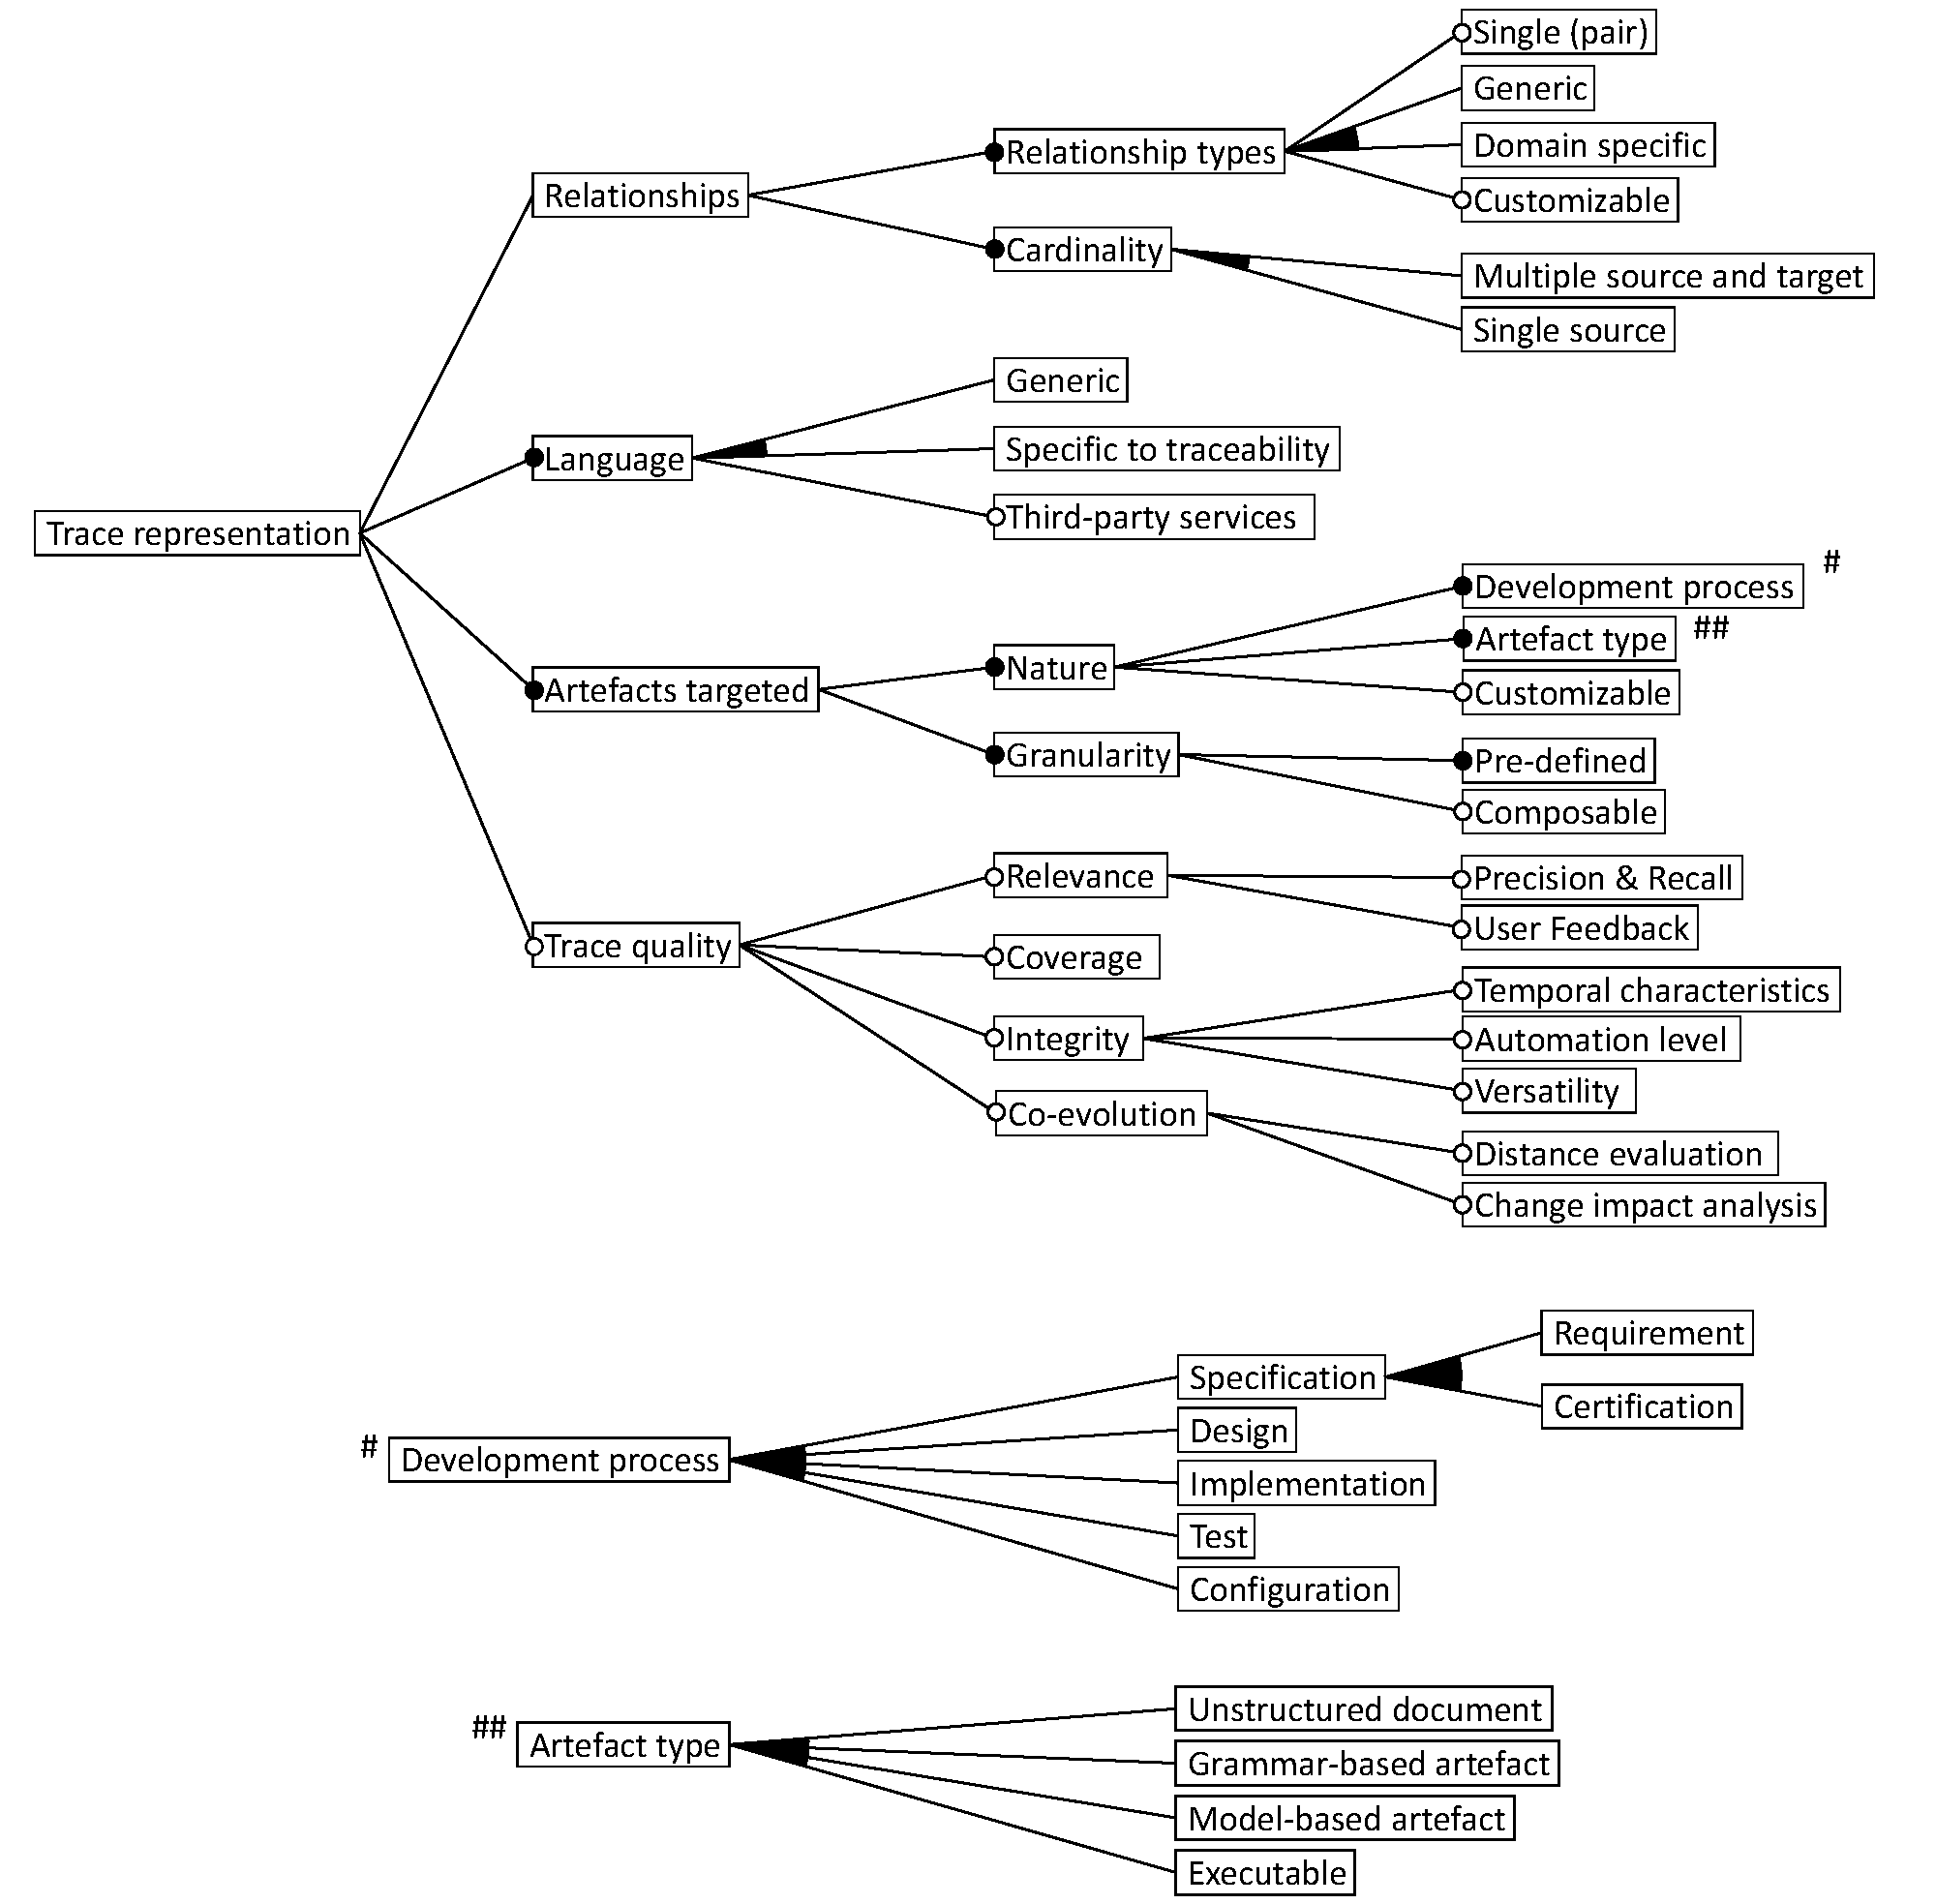
\includegraphics[width=.90\linewidth]{images/fm-definition}
	\caption{Features related to the representation of a trace.}
	\label{fig:fm:definition}
\end{figure}


As discussed in the terminology section, there is no common representation or standard of traceability. Instead, we find a plethora of applications of traceability on specific domains such as program understanding, with approaches facilitating the localisation of features~\cite{seiler2019-comparing-trac-through-IR-Commits-Logs} and bugs~\cite{ko2008-whyline-debugging}, software decomposition into relevant partitions~\cite{laghouaouta2017-model-composition-tracaebility} or slices~\cite{nejat2012-traceability-sysml-safety-certification}, software reuse ~\cite{tinnes2019-improving-art-reuse-with-traceability}, and for supporting general explainability of the software process and product~\cite{wohlrab2020-traceability-organization-process-culture}. 


In each of these scenarios, traces are used to support debugging or to help gather evidences for certification. And for that, all approaches present their tailored representation for trace artefacts. The very notion of trace as well as their aim differ from one perspective to another. %If this hampers the emergence of a common knowledge, it has the value to explore the potential features to automate inlined with the needs from application domains. 
Researchers present generic graph-based representations particularly suitable for model-based environment~\cite{schwarz2010-graph-based-traceability,grammel2012-model-matching-for-traceability-in-MDE} ; while others focus on  the verification and validation of software artefacts~\cite{Dubois_2010,vonknethen2002-change-oriented-req-traceability-evolution-of-embedded-systems} and traceability artefacts~\cite{rempl2014-conformance-of-traceability-to-guidelines} ; and others target the maintenance of software systems with representations for change impact analysis~\cite{goknil2014-change-impact-analysis-for-requirement-metamodel} or multi-model consistency~\cite{Szabo_2013}. Representations are so diverse that our survey selected more than 80 papers mentioning their own distinct definitions for trace-based approaches, with 41 metamodels effectively depicted. 
%\eb{So many perspectives shall provide enough details for a standard, or at least a common understanding (cf our metamodel?).}


\Fig{fig:fm:definition} shows the hierarchy of features related to the definition and the representation of trace artefacts. A peculiar focus is put on the typing of relationship. this figure an important feature to allow for traceability applications to specific domains in their own language. We detail as well variability in the language used and the artefacts targeted by traceability approaches and explore the needs for more quality measurement and assessment of trace artefacts.


\paragraph{Artefacts targeted} 
In relation to the artefacts targeted by traceability purposes we distinguish between the nature of the artefact and its granularity as both dimensions are important and used in the literature. For the nature, on the one hand, investigations differ on the development phase they target. Link between requirement specifications to design and code level predominate the literature with more than 50\% of the papers found in the survey addressing requirement traceability. Other phases as well are targeted such as test and verification in a lesser proportion. On the other hand, the type of the artefacts is important to deduce the level of generalization transversal to the development lifecycle. Papers focus on four different types: unstructured document, grammar-, and model-based artefacts, and binaries.
For artefacts granularity, if there exist attempts to a generalizable approach were the granularity of artefacts (their level of decomposition) is customizable (\textit{e.g.,} by polymorphism), others only focus on a specific type to accentuate the scrutiny on specific optimizations of the execution of traceability features.


\textbf{Tracing model-based development}
Our selection shows numerous publications referring to the application of tracing features to model-based approaches. As authors report, the use of MDE tooling such as ATL~\cite{Santiago_2013,Jim_nez_2013}, or the Eclipse Modeling Framework (EMF) allows the automated generation of traceability information as a side effect of executing operations~\cite{galvao2007-survey-traceability-in-MDE,winkler2010-survey-traceability-and-MDE}. 
As a matter of fact, among the 41 metamodels selected by the survey, there are generic metamodels for end-to-end traceability~\cite{heisig2019-generic-traceability-metamodel-end-to-end-capra,Haidrar_2016}, as well as metamodels specific to engineering domain such as model transformation~\cite{Jim_nez_2013,anquetil2010-model-driven-tracea-for-SPL,vara2014-traceability-in-MDD-MTransfo} or software product line~\cite{Jim_nez_2013,vara2014-traceability-in-MDD-MTransfo}. 
The Requirement Interchange Format (ReqIF) is an attempt to standardise requirement tracing in the EMF community~\cite{Graf_2012}.
Yet, industry has not standardised on EMF - they use a wide variety of technologies for modeling, and some of it does not conform to the usual notions of modeling technology: they may not have explicit metamodels.
Paige \textit{et al.} offer to address this issue in a call for more flexible modeling where models of different formats are associated to each other with annotations that allow automated bond or dependency inference between both application and engineering domains~\cite{seiler2019-comparing-trac-through-IR-Commits-Logs,paige2017-changing-mde}.



\paragraph{Language (genericity)} 
The choice of the implementation language will impose constraints that must be evaluated beforehand. Studies presenting work related to the development of languages for traceability are legion. Some authors attempt a generic definition of traceability~\cite{heisig2019-generic-traceability-metamodel-end-to-end-capra,azevedo2019-traceability-metamodel-and-reference-model}, whereas others concentrate on specific uses such as SysML adaptation~\cite{nejat2012-traceability-sysml-safety-certification}, or SPL traceability~\cite{anquetil2010-model-driven-tracea-for-SPL}. 
Languages specific to traceability provide the ability to represent trace artefacts with increased relevance and accuracy. Yet, they often suffer the limitation to be built \textit{ad hoc} and lack a significant power of generalization.

We found few studies interested in the use of generic software language for traceability - even though industrial partners are interested with legacy software instrumentation for traceability and thus would benefit from traceability project coded in their legacy language~\cite{nejat2012-traceability-sysml-safety-certification}. Representing traces in spreadsheets, text files, or databases offers greater freedom of expression than using a domain specific language. This is due to the nature of actors in software development and the cognitive gap that remains between software engineers and experts of other domains. 
The maintenance costs turns out to grow accordingly and team members fail to update the trace artefacts~\cite{clelandhuang2007bestPracticeForAutomatedTraceability}.

\paragraph{Relationship types} 
As many authors have demonstrated, the ability offered to the user to define personalized types of relations between the artefacts of a system fosters the comprehensibility of the traces produced. We distinguish between approaches offering predefined types, most often relating to the field of software engineering (implements, inherits, uses, executes ...) and approaches allowing a domain specific typing. The formers allow increased monitoring and user-friendliness \textit{for IT experts}. They are not very attractive to \textit{experts in other sectors}. 
Allowing users to define the types of relationships specific to their area of expertise helps to fill in the cognitive gap that separates the design from the use of tracing functionalities~\cite{olive2002-representation-of-generic-relationship-types-in-modeling} - and the communication gap that lies between respective communities~\cite{wohlrab2020-traceability-organization-process-culture}.

SysML v2, tries to formalize traceability relationships more clearly, rather than just using a dependency-like mechanism. A emphasis is put on requirements with the definition of mechanisms in the concrete syntax to check their satisfaction~\cite{Haidrar_2016}.  

Publications focusing on trace identification rarely consider other types of artefacts than the peculiar pair their optimisation target.

The literature shows also a distinction between approaches considering relationships with multiple sources and targets and relationships allowing only a single source.  


\paragraph{Trace quality} 
In most of the papers we studied, quality aspects were barely mentioned. The relevance of traces, their coverage of the (part of) the system they target, their integrity or versatility have been long due for in depth investigation and standardization. The relevance of trace artefacts is mainly evaluated with precision and recall measurements while few researchers include a user feedback~\cite{clelandhuang2014-traceability-trends-and-futurte-direction}. Their coverage is considered an important characteristics in approaches to software testing~\cite{gannous2019-Certification-into-Model-based-Testing-for-Safety-Critical-Systems}. It is also used by Rath \textit{et al.} who address the fundamental problem of missing links between commits and issues. They train a classifier with textual commit information to identify missing links between issues and commits (\ie a lack in the coverage)~\cite{rath2018-guo-augmenting-incomplete-traces}. Integrity of traces is addressed in work on model transformation where co-evolution figures an automatic verification of their coherence with other (versatile) software artefacts~\cite{Szabo_2013,slotosch2018-Modeling-and-Certification-of-MDD-Processes}. 
The co-evolution of traces implies measuring some kind of distance between artefacts (syntactic, cognitive, geographic, cultural...)~\cite{bjarnasson20016-theory-of-distances-in-SE}.  It also refers to the analysis of the changes of the system that impact traceability artefacts~\cite{goknil2014-change-impact-analysis-for-requirement-metamodel,vonknethen2002-change-oriented-req-traceability-evolution-of-embedded-systems}. In our survey, nine papers address artefacts co-evolution and 17 tackle model transformation limitations. These latter figuring a valuable tool to automate co-evolution tasks. The other quality concerns are left for future work and remain mainly an open issue.

A few publications relate the quality of their work on the computation of aggregated values, evaluated against company (or project specific) thresholds~\cite{Bunder_2017_query-for-quality}. They make use of rules to automate the computation of customizable analyses and show that query, metric and rules are a powerful combination to do so.
There is a need to understand clearly the purpose of trace-based approaches to define explicit measurements to evaluate traces accuracy, relevance, and deterioration.

\subsubsection{Trace identification}
\label{sec:fm:identification}
\begin{figure}[h]
	\centering
	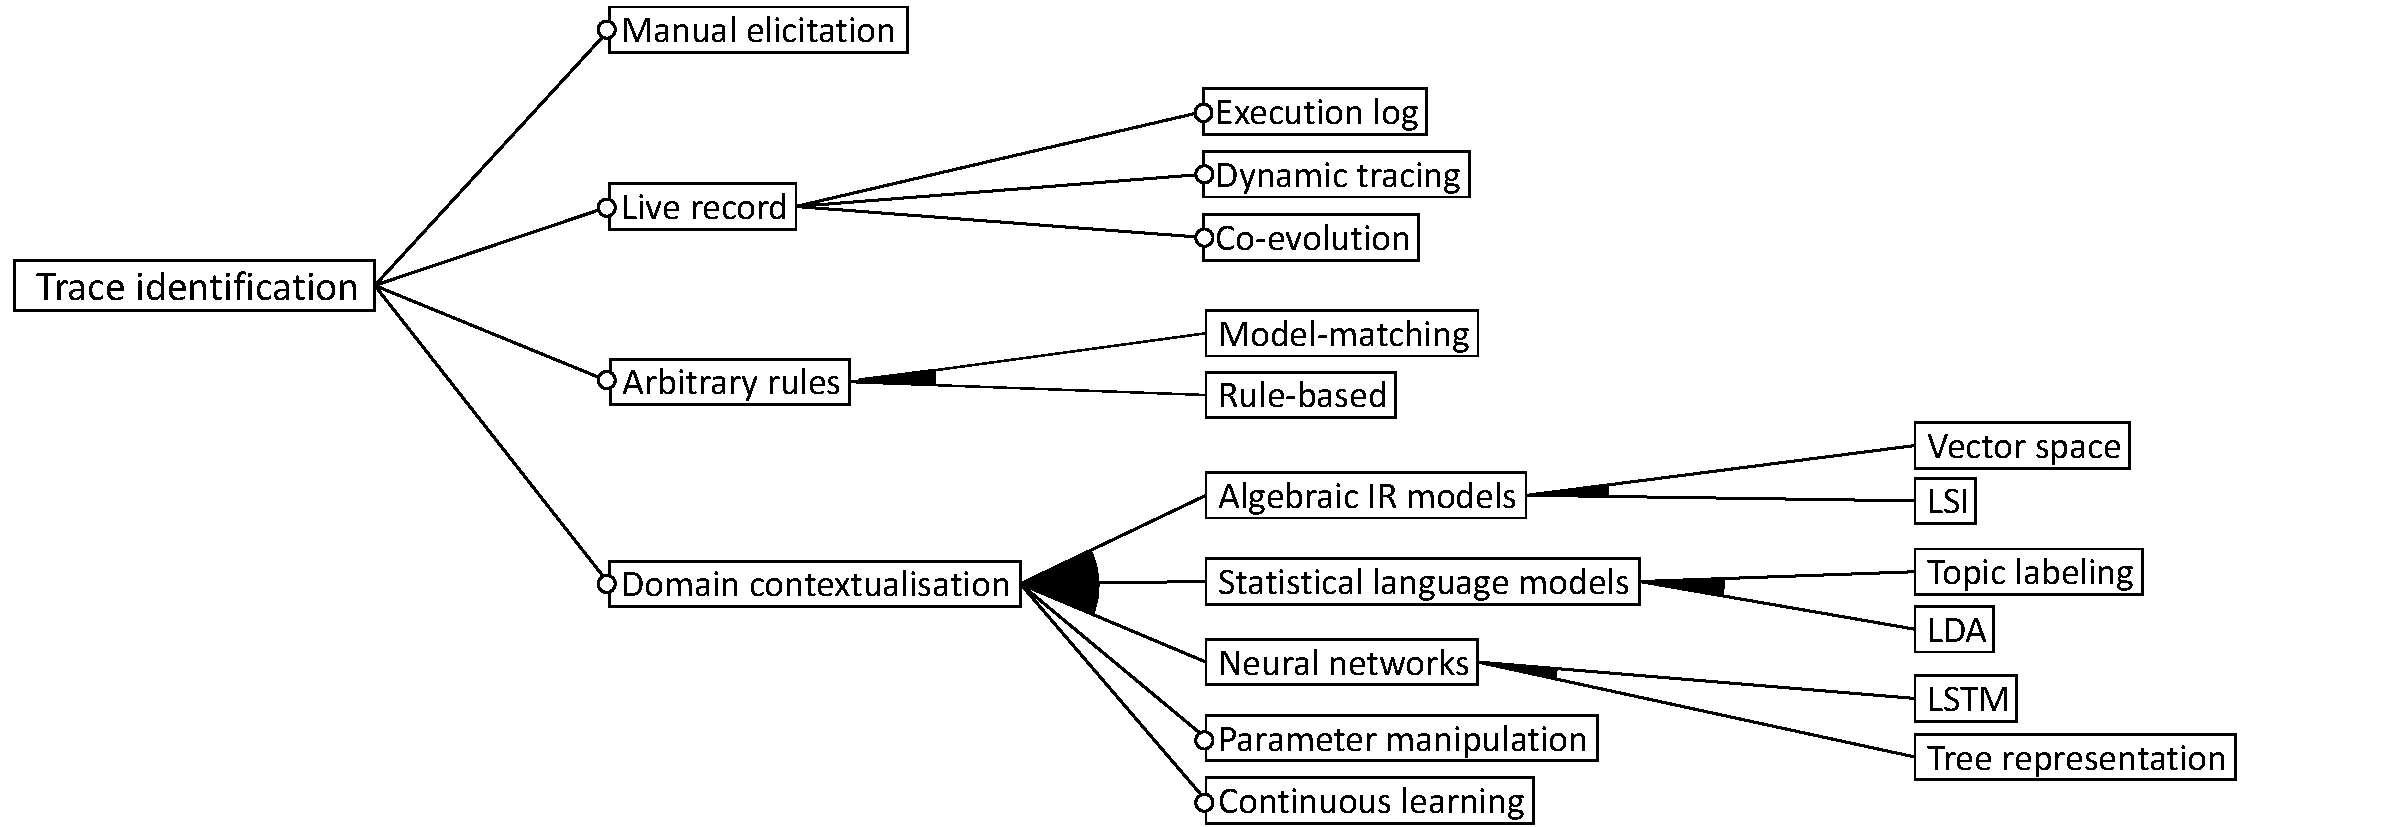
\includegraphics[width=.99\linewidth]{images/fm-identification}
	\caption{Features related to the identification of trace links}
	\label{fig:fm:identification}
\end{figure}

%Many publications tackle the difficulty to automate the identification of trace links and introduce approaches based on the application of natural language processing techniques. 
\Fig{fig:fm:identification} shows the hierarchy of features related to the identification of traces: 
the manual elicitation of traces, 
their live record during execution and evolution,
rule-based alternatives to assist the user with automation potential, 
and AI-augmented identification with domain contextualization.



\paragraph{Manual elicitation and recording instrumentation} 
Manual elicitation makes possible to create traces in an \textit{ad hoc} manner. As an example, our industrial partner chose to hire a developer to elicit trace links necessary for a certification commitment. This was chosen rather than a (semi-)automated approach.

Teams investigate as well the {live record} of traces during the execution and the evolution of software artefacts. There are initiatives to instrument existing languages such as ATL with rich log generation~\cite{Santiago_2013,la_Fosse_2018}, while others consider trace record an aspect that can be plugged on current existing languages~\cite{Pfeiffer_2014,Santiago_2013}. Ziegenhagen \textit{et al.} mix execution traces with metadatas~\cite{ziegenhagen2020-expanding-tracea-with-dynamic-tracing-data}, and use developer interaction records~\cite{ziegenhagen2019-developer-tool-interaction} to enrich existing traceability artefact.

Model transformations are considered the hearth and soul of MDE and, consequently, numerous studies attempt to enrich trace generation during transformation execution~\cite{vara2014-traceability-in-MDD-MTransfo,Saada_2013,la_Fosse_2018}. This allows a semantically rich tracing of target and source artefacts~\cite{paige2011-traces-in-moel-driven-engineering}. 



\paragraph{Use of arbitrary rules} 
%Once a system is in place, the links that one might want to use (for locating features, increasing code understanding, and reducing perpetual maintenance effort) can be partly recovered automatically. Indeed, the knowledge that programmers process when writing the code is often captured by the mnemonics for identifiers~\cite{antoniol2002-tracing-code-documentation-links}. The analysis of these mnemonic means allows the constitution of linkage rules between software artefacts. The example of the similarity between Java classes file names and their respective binaries is obvious. 
Teams identify rules that help retrieve and maintain traceability relations~\cite{mader2008-rule-based-maintenance-post-requirements-traceability,spanoudakis2004-rule-based-generation-of-req-traceability-relations}.
Antoniol \textit{et al.} use the mnemonics for identifiers to establish trace identification rules~\cite{antoniol2002-tracing-code-documentation-links}.
At the model level, Grammel \textit{et al.} use a graph-based model matching technique to exploit metamodel matching techniques for the generation of trace links for arbitrary source and target models~\cite{grammel2012-model-matching-for-traceability-in-MDE}, and Saada \textit{et al.} recover  execution traces of model transformation using genetic algorithms~\cite{Saada_2013}.


\paragraph{Domain contextualisation} 
Borillo \textit{et al.} published a precursor article on the use of information retrieval techniques for linguistics applied to spatial software engineering. They opened the box for AI-augmented traceability~\cite{borillo1992-linguistic-engineering-to-spacial-SE}. 
Today, domain contextualization with means of machine learning for topic modeling, word embedding, and more generally knowledge extraction from unorganized text documents is the most studied feature of traceability~\cite{guo2017-semantically-enhanced-tracebility-deep-learning,wohlrab2020-traceability-organization-process-culture}. We found 22 approaches dedicated to this topic in our survey. 

Researchers first extracted word vectors from natural language artefacts to take account of the neighbouring words a term in the application domain may relate to~\cite{delucia2012-information-retrieval-for-traceability}. This effort made the identification of bonds between requirement specifications and other artefacts possible with a gradually improving precision. Since then, many other information retrieval techniques for natural language processing were applied with success~\cite{arunthavanathan2016-traceability-with-NLP}. Studies on domain contextualization are separated into three subgroups according to the type of tools used (algebraic information retrieval models, statistical language models, and neural network).  For example, Florez \textit{et al.} derivate fine grained requirement to source code links~\cite{florez2019-finegrained-req2code}, Rath \textit{et al.} complete missing links between commits and issues~\cite{rath2018-guo-augmenting-incomplete-traces}, Marcus \textit{et al.} identify links between documentation and source code~\cite{marcus2003-latent-semantic-indexing-for-traceability-LSI}. An interesting publication from Poshyvanyk \textit{et al.} shows that mixing expertize both in information retrieval techniques and engineering domains gives far better results than expertizes taken separately (they exemplify their theory with feature localization). 
Teams are also using genetic algorithms to cope with the variety of algorithms and parameters these approaches use~\cite{marcen2020-req2model-with-EA-ranking-train-system,panichella2013-genetic-programming-for-effective-topic-modeling}, and structural information to foster methodologies interweaving~\cite{panichella2013-using-structural-information-to-improve-IR-traceability}. Unfortunately, a common critique rose against these positive results. Too many teams compete with each others to accomplish better quantified precision and recall when too few attempt at qualifying the overall relation between these measurement and the effective impact on software development~\cite{clelandhuang2014-traceability-trends-and-futurte-direction,shin2015-guidelines-benchmark-auto-traceability}. 
%Ultimately, the reach for an ideal end-to-end automated traceability has led research, with the buzzing of AI, into a technical competition where teams compete with each others to beat the state-of-the-art Precision\&Recall for link identification between text artefacts~\cite{shin2015-guidelines-benchmark-auto-traceability}. 
%Despite authors enthusiasm about their results, 
Borg \textit{et al.} conclude their systematic literature mapping on information retrieval approaches to traceability noticing that there are no empirical evidence that any IR model outperforms another model consistently~\cite{borg2014-SmS-IR-for-traceability}. 

The ability to continuously improve the learning process is mentioned in the literature but we found no evidence of its application. 
Whereas all study tend to focus on the identification of trace links, Rosenkranz \textit{et al.} investigate the impact of language quality for the retrieval of information~\cite{Rosenkranz_2013}.

%Marcen \textit{et al.} use machine learning to rank configurations for the execution of these techniques on specific applications~\cite{marcen2020-req2model-with-EA-ranking-train-system}. Marcen \textit{et al.} use evolutionary algorithms to rank machine learning algorithm parametrization according to their performance in trace retrieval for a specific application. 

\subsubsection{Trace management}
\label{sec:fm:toolsupport}
\begin{figure}[h]
	\centering
	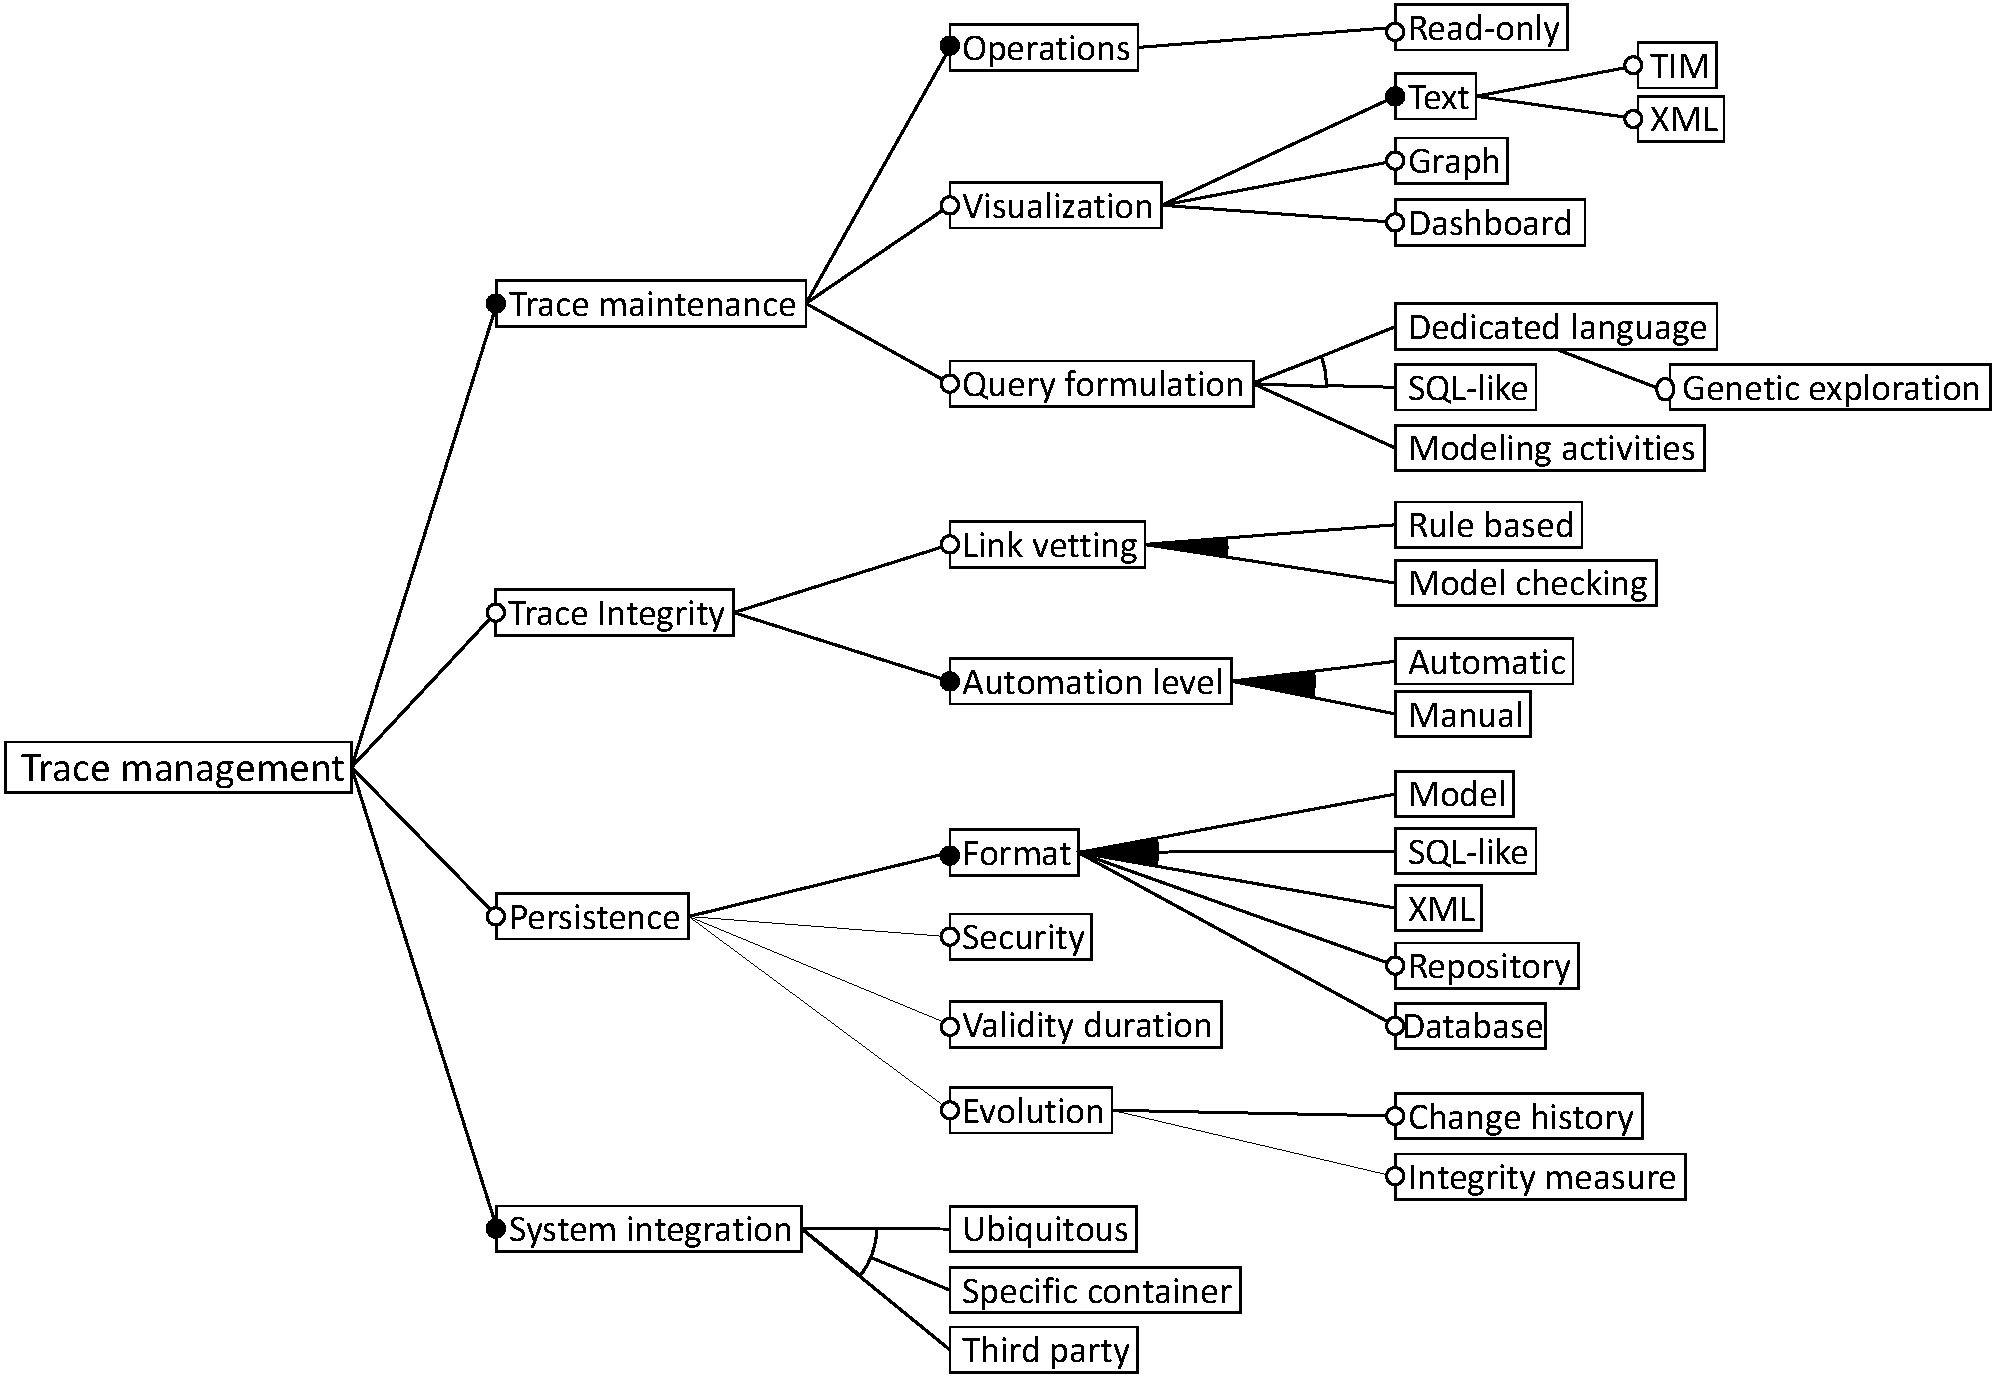
\includegraphics[width=.9\linewidth]{images/fm-toolsupport}
	\caption{Tool support for traceability management.}
	\label{fig:fm:management}
\end{figure}

%Our survey shows how numerous and different are the purposes of traceability. They span through the entire software lifecycle and involve all levels of abstraction -- from textual notes to high-order modelling artefacts everything that could be potentially required for software development and maintenance. %A clear understanding of traceability at all levels of the software development would help motivate teams in the edification of a common knowledge~\cite{mader2009-motivation-matters-in-traceability-practitioner-survey}. 
%There exist basic commonalities and variabilities shared among traceability approaches. to draw a general map of the techniques that traceability approaches use to store and maintain trace artefacts. 

\Fig{fig:fm:management} shows the hierarchy of features related to the management of trace artefacts. We distinguish between the actual maintenance of trace artefacts, the evaluation of their integrity, the means of persistence, and the level of integration in software systems.

\paragraph{Trace Maintenance} 
Trace links suffers a gradual decay that must be considered seriously to avoid having to re-elicit traces every time they need be analysed. A manual maintenance is out of reach for the amount of information such inspections would involve is enormous. This motivates a serious consideration of automated ways to visualise and retrieve them. 
%The vast amount of potential trace links traceability approaches have to handle motivate a serious consideration of automated ways to visualise and retrieve them. 
Co-evolution techniques~\cite{mader2008-rule-based-maintenance-post-requirements-traceability,drivalos2010-state-based-traceability} and visualization initiatives~\cite{fittkau2013-explorviz-Trace-Visualization} attempt to tackle the burden to maintain trace links up-to-date~\cite{seibel2010-dynamic-hierarchical-models-comprehensive-traceability,Bunder_2017_query-for-quality}. 

More precisely, structured text, in the form of metamodel instances or XML sheets allows query-based mining of trace datasets. Hyper-text links is a \textit{de facto} standard to browse trace links. Indeed, following links branches through successive clicks has become almost natural. The use of graphical representations stimulate human perception and the integration of such technique in traceability frameworks is a useful feature to augment tracing awareness. Successful dashboards offer to show simultaneously and synchronously multiple perspectives~\cite{ruiz18-traceME-conceptual-model-evolution,santiago2013traceability-in-MDE,heisig2019-generic-traceability-metamodel-end-to-end-capra}.
In parallel, allowing a rich formulation of queries to assist the exploration of existing traces will help reducing the amount of information users need to navigate through~\cite{Bunder_2017_query-for-quality,dietrich2013-learning-efective-query-transformation-for-enhanced-req-trace-retrieval}. Querying depends on the type of representation of traceability artefacts. SQL-like languages benefit from a long history of information mining while dedicated languages offers better legibility. Genetic programming has also permitted the automation of query formulation. Finally, model matching can be used to filter interesting traces from a repository.

All in all, assisting efficiently end-users in the retrieval, visualization and analysis of traces is not easily granted. Yet, studies on the topic remain scarce in comparison to other concerns. There is still great space for improvement and calls for more work in that direction are redundant through literature studies~\cite{Gotel2012,antoniol2017-traceability-grand-challenges}.

\paragraph{Trace Integrity} 
To cope with the volatility of software products and processes, the integrity of traces must be given due consideration. Work on these questions, although called out loudly by literature studies, is scarce in practice. The first option is given with manual annotation, or vetting of trace links to inform about their level of reliability. Annotations allow a qualitative and quantitative evaluation~\cite{Buchmann_2015}. This is the case for a back-propagation of verification and validation results between design and requirements~\cite{Hegedus_2010}.  
Another approach is to impose invariant rules while manipulating traces or their targets~\cite{Bunder_2017_query-for-quality}. For example, when a change occurs in an artefact targeted by a trace, if the corresponding link was identified more than two versions prior to the current version, issue an alert. 
Teams set up co-evolution processes to ensure the coherence of the trace is maintained~\cite{rahimi2019-Evolving-trace-req2source}. 


\paragraph{Trace persistence} 
Many different storages alternatives exist for traceability artefacts.
An option is to use SQL-like grammar to store and retrieve traces with the power of database tooling, or to use XML documents to represent trace matrix in a transformable format. The industry uses a lot of informal format and link representations often remain implemented in spreadsheets, text files, databases or requirement management tools. These links deteriorate quickly during a project as time pressured team members fail to update them. Researchers aiming at a generalizable approach favour model-based representations able to express specifically defined concepts related to traceability (often in a specific domain of application)~\cite{clelandhuang2007bestPracticeForAutomatedTraceability}. The burden of maintaining traces coherent is eased in model-based solutions.

Another concern lies in the recording of trace evolution. The trace creation should be recorded, with the successive changes that affect it. Integrity measures respective to these time stamps should be recorded as well to evaluate their evolution during a period of time. Yet, we did not found any paper addressing explicitly this issue.
Considering that traceability has become a major quality for certification, it is surprising to see very little interest in security concerns related to trace artefacts either.


\paragraph{System integration} 
Helming \textit{et al.} use of the same modeling language for both traceability and system artefacts~\cite{helming2009-traceability-change-awareness}. The conjunct use of EMF and a dedicated traceability metamodel (both written in Ecore) facilitates the integration of traceability features including graphical versions to stimulate human perception and standard analysis of traces in the native environment of the traced system. 

On the other hand, Galvao \textit{et al.} in their seminal work on traceability and MDE call for a loosely coupled traceability support that can integrate external relationship with independent representations (in another, ideally common language)~\cite{galvao2007-survey-traceability-in-MDE}. To our knowledge, the most advanced research in this direction was published by Azevedo \textit{et al.}~\cite{azevedo2019-traceability-metamodel-and-reference-model}. 


%\subsection{Traceability purposes}
%\label{sec:traceablitypurposes}
%Our survey shows how numerous and different are the purposes of traceability. They span through the entire software lifecycle and involve all levels of abstraction -- from textual notes to high-order modelling artefacts everything could be potentially required for software development and maintenance. A clear understanding of traceability at all levels of the software development would help motivate teams in the edification of a common knowledge~\cite{mader2009-motivation-matters-in-traceability-practitioner-survey}. Yet, this sharing is slow to come. It is in part due to the fact that is hard to define measurements in software engineering, and metrics must be clearly understood to be shared and compared in order to reproduce experiments and foster research~\cite{bjarnasson20016-theory-of-distances-in-SE}. In each and every application domain, a clear goal, a detailed purpose, allowing for a neat quantification of the progress made with traceability would help teams predict and measure the benefit they can expect from traceability approaches~\cite{mader2013-strategic-traceability-for-safety-critical-projects}.
%%The emergence of a standard would help establish distance measurement tailored to traceability, and would foster its control and automation rate.
%To engage toward the emergence of this ideal common standard, we propose an explicit breakdown of the knowledge area covered by these different approaches. As can be seen in \Fig{fig:knowledgearea}, the ability to trace artefacts of a software system is recognized as a good support to enhance software analysis, maintenance, and certification. This broad decomposition shall help perceive the variability in the vocabulary of traceability investigations. 
%
%
%\begin{figure}[h]
%	\centering
%	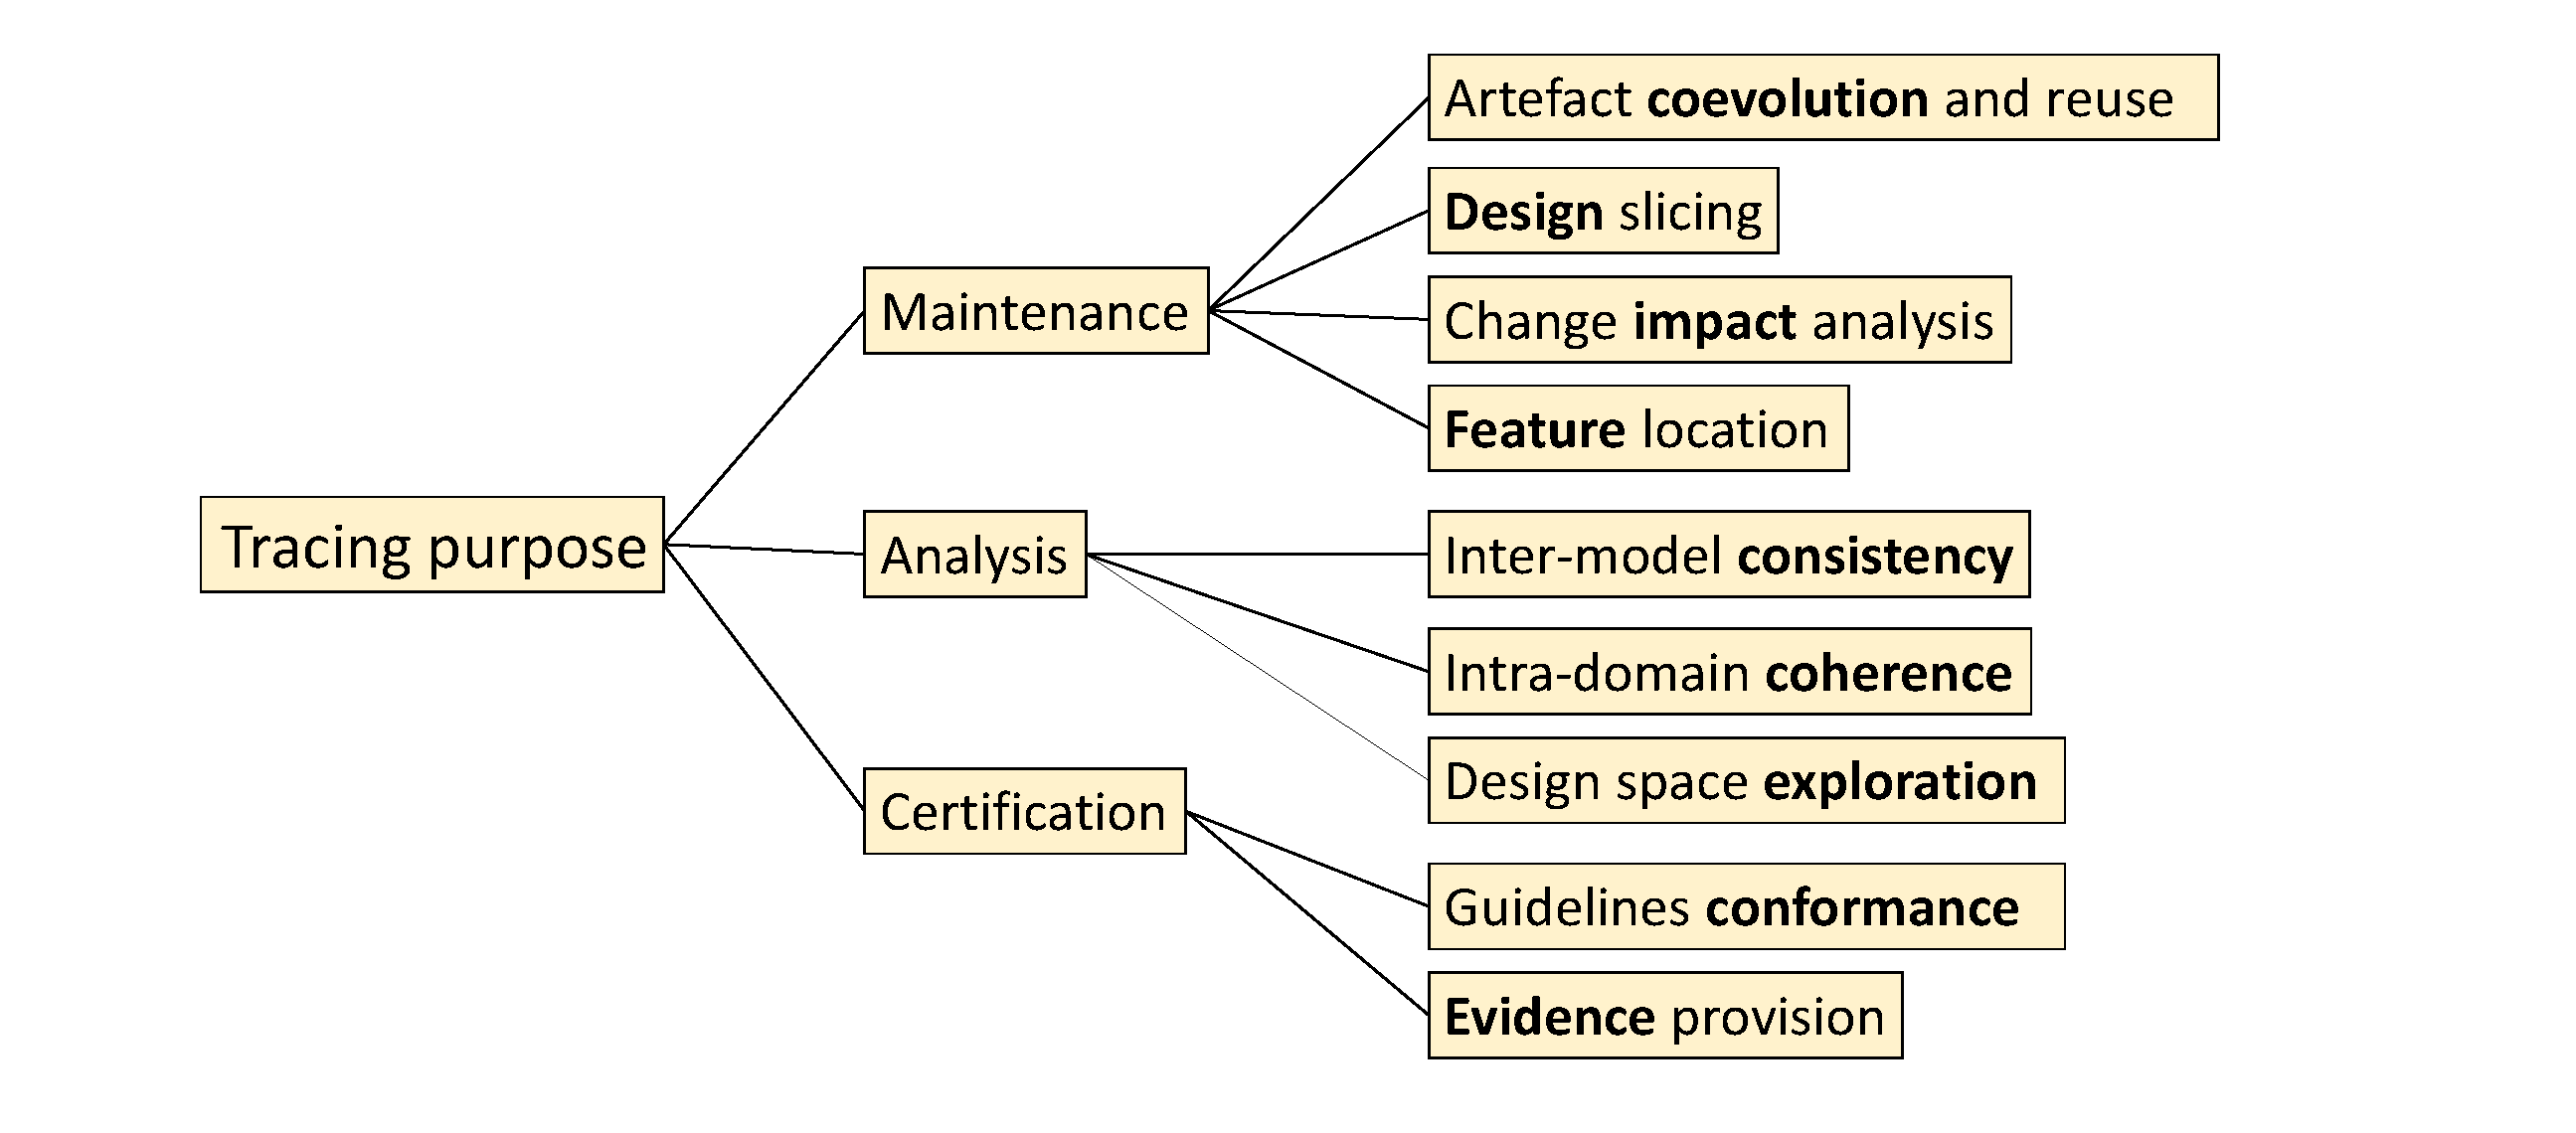
\includegraphics[width=.7\linewidth]{images/fm-tracingpurpose}
%	\caption{Traceability purposes. }
%	\label{fig:knowledgearea}
%\end{figure}
